Aufgrund des Umfangs der Blocklib und der Unübersichtlichkeit an einigen Stellen, die beispielsweise durch die Klasse \classContext{} entsteht, kann das Jobsystem nicht auf die in Abbildung~\vref{fig:optimalArchitecture} gezeigte Art  integriert werden. Um dennoch die Anforderungen von Kapitel~\ref{sec:anforderungen} zu erfüllen, wird daher ein Jobsystem implementiert, das nur an Stellen mit der Blocklib konsolidiert wird, die bereits zuvor Multithreading genutzt haben (siehe Tabelle~\ref{tab:concTasksBlocklib}), und ansonsten für die zukünftige Nutzung bereitsteht.

\begin{figure}
	\centering
	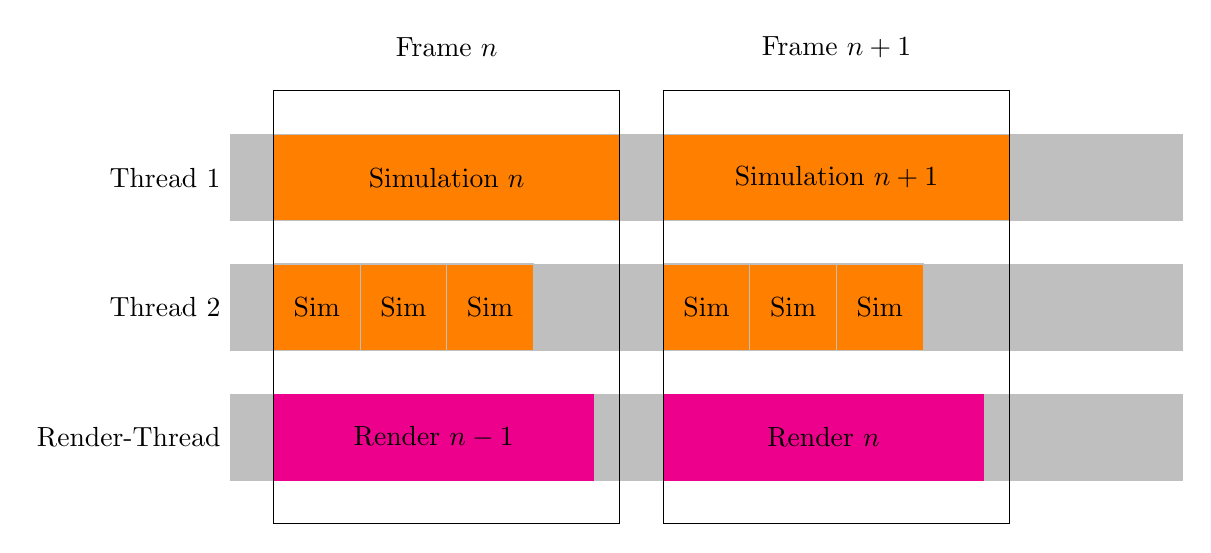
\begin{tikzpicture}[scale=1.1]
		\fill[lightgray]  (0,0) rectangle (11,1);
		\fill[lightgray] (0,-1.5) rectangle (11,-0.5);
		\fill[lightgray]  (0,1.5) rectangle (11,2.5);
		
		\node[anchor=east] at (0,2) {Thread 1};
		\node[anchor=east] at (0,0.5) {Thread 2};
		\node[anchor=east] at (0,-1) {Render-Thread};
		
		
		\fill [orange,draw=lightgray] (0.5,1.5) rectangle node[black] {Simulation $n$} (4.5,2.5);
		\fill [orange,draw=lightgray] (0.5,0) rectangle node[black] {Sim} (1.5,1);
		\fill [orange,draw=lightgray] (1.5,0) rectangle node[black] {Sim} (2.5,1);
		\fill [orange,draw=lightgray] (2.5,0) rectangle node[black] {Sim} (3.5,1);
	
		\fill [orange,draw=lightgray] (5,1.5) rectangle node[black] {Simulation $n+1$} (9,2.5);
		\fill [orange,draw=lightgray] (5,0) rectangle node[black] {Sim} (6,1);
		\fill [orange,draw=lightgray] (6,0) rectangle node[black] {Sim} (7,1);
		\fill [orange,draw=lightgray] (7,0) rectangle node[black] {Sim} (8,1);
	
		\fill [magenta] (0.5,-0.5) rectangle node[black]{Render $n-1$} (4.2,-1.5);
		\fill [magenta] (5,-0.5) rectangle node[black]{Render $n$} (8.7,-1.5);
		
		\node at (2.5,3.5) {Frame $n$};
		\node at (7,3.5) {Frame $n+1$};
		
		\draw  (0.5,3) rectangle (4.5,-2);
		\draw  (5,3) rectangle (9,-2);
	\end{tikzpicture}
	\caption[Design der neuen Multithreading-Architektur der Blocklib.]{Design der neuen Multithreading-Architektur der Blocklib. Statt einer Simulation, die vollständig aus Jobs besteht, gibt es einen langen Simulations-Job, der die meisten Anweisungen sequentialisiert ausführt, aber weitere Jobs starten kann, die Teile der Simulation nebenläufig ausführen. \enquote{Sim} kennzeichnet einen solchen nebenläufigen Simulations-Job.}\label{fig:plannedArchitecture}
\end{figure}

Da die Blocklib nicht vollständig umstrukturiert wird, um ein Jobsystem zu nutzen, verändert sich der Entwurf der nebenläufigen Architektur konzeptuell. Nun erinnert die Architektur stärker an \ac{sot} als an ein Jobsystem. Diese Änderung ist in Abbildung~\vref{fig:plannedArchitecture} zu sehen. Anstatt die gesamte Simulation in viele kleine Jobs zu zerlegen, bleibt ein langer sequentialisierter Simulations-Job bestehen, der dann aber die Möglichkeit besitzt, weitere nebenläufige Jobs zu starten. Mit dieser Architektur ist es möglich, die Blocklib inkrementell zu der in Abbildung~\vref{fig:optimalArchitecture} gezeigten Architektur umzuwandeln, indem in zukünftigen Arbeiten immer mehr pseudo-sequentialisierte \glspl{Anweisung} der Simulation als nebenläufige Jobs definiert werden, bis sie vollständig aus Jobs besteht. So kann die Architektur, mit Ausnahme des Render-Threads, dynamisch von hauptsächlich \ac{sot} zu einem Jobsystem wechseln.

Java bietet mit dem Interface \classScheduledExecutorService{} bereits eine gute und bekannte Schnittstellendefinition, die für ein Jobsystem genutzt werden kann. Daher baut das Design des Jobsystems der Blocklib auf diesem Interface auf. 

\begin{figure}
	\includesvg[width=\textwidth]{GrobesDesign.svg}
	\caption[Struktur des entwickelten Jobsystems.]{Struktur des entwickelten Jobsystems. Das in der Blocklib definierte Interface wird von dem Interface \classScheduledExecutorService{} abgeleitet. Damit steht ein für Java-Entwickler bekanntes Interface bereit, das erweitert wird.}\label{fig:GrobesDesign}
\end{figure}

In Abbildung~\vref{fig:GrobesDesign} ist die Struktur des Entwurfs für das Jobsystem der Blocklib dargestellt. Es wird ein Interface \classBlocklibExecutorService{} definiert, das von dem Interface \classScheduledExecutorService{} der Java-Bibliothek abgeleitet ist. Das Interface wird so erweitert, dass die verschiedenen \code{submit(...)}-Methoden jeweils Objekte des Typs \classCompletableFuture{} zurückgeben. Die \code{schedule(...)}-Methoden geben jeweils ein \classScheduledCompletableFuture{}-Objekt zurück, das später noch näher erläutert wird.

Das Interface \classBlocklibExecutorService{} wird durch die Klasse \classBlocklibExecutor{} implementiert. Sie nutzt zur Durchführung von Jobs den von der Java-Bibliothek definierten \classScheduledThreadPoolExecutor{}. Um die für die Rückgabewerte nötigen \classCompletableFuture{}-Objekte zu erzeugen, wird eine Klasse \classCompletableFutureWrapper{} erstellt. Eine vollständige Auflistung der von den drei Interfaces bereitgestellten Methoden ist in Anhang~\vref{appendix:BlocklibExecutorService} zu finden. 

Die \acs{api} des Jobsystems bietet verschiedene Methoden, um nebenläufige \glspl{Anweisung} zu starten. Mittels der \code{submit(...)}-Methoden können \glspl{Anweisung} definiert werden, die sofort nebenläufig ausgeführt werden. Da diese Methoden ein \classCompletableFuture{}-Objekt zurückgeben, lassen sich über die dort definierten Methoden (siehe Anhang~\vref{appendix:CompletionStage}) einfach nachgelagerte nebenläufige \glspl{Anweisung} definieren, die abhängig von der Vollendung der ursprünglichen \gls{Anweisung} ausgeführt werden. Mit den \code{schedule(...)}-Methoden wird analog dazu eine Möglichkeit geboten, \glspl{Anweisung} zu definieren, die nach Ablauf eines bestimmten Zeitintervalls nebenläufig ausgeführt werden. Mittels \code{scheduleAtFixedRate(...)} und \code{scheduleWithFixedDelay(...)} können periodisch durchzuführende \glspl{Anweisung} gestartet werden.